\documentclass[tikz,border=10pt]{standalone}
% No extra TikZ libraries are needed for this figure.
\begin{document}
% Scale: s = 0.010444 cm/px, origin at A (123,795) px; y flipped.
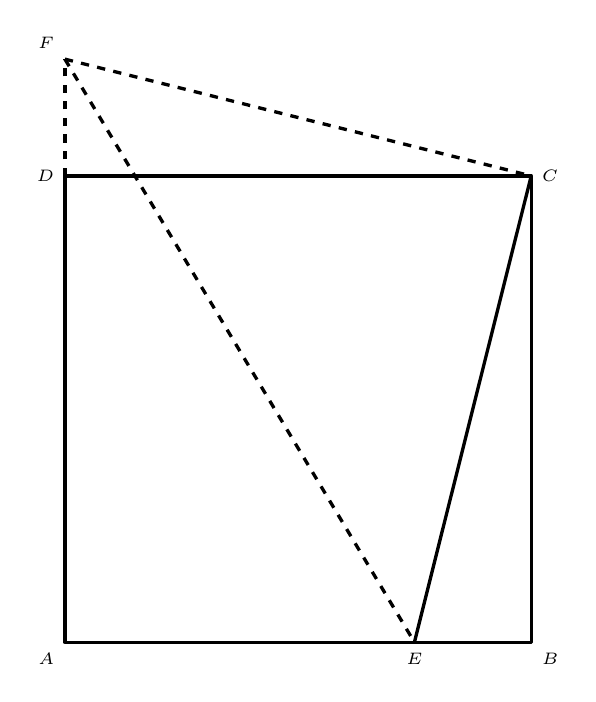
\begin{tikzpicture}[line width=1.2pt, line join=round]

% Named coordinates
\coordinate (A) at (0,0);        % (123,795) px
\coordinate (B) at (5.922,0);    % (690,795) px
\coordinate (C) at (5.922,5.922);% (690,228) px
\coordinate (D) at (0,5.922);    % (123,228) px
\coordinate (E) at (4.439,0);    % (548,795) px
\coordinate (F) at (0,7.405);    % (123,86) px

% Square ABCD (solid)
\draw (A) -- (B) -- (C) -- (D) -- cycle;

% Solid segment CE
\draw (C) -- (E);

% Dashed segments DF, FE, FC
\draw[dashed] (D) -- (F);
\draw[dashed] (F) -- (E);
\draw[dashed] (F) -- (C);

% Labels (6pt font from STYLE METRICS)
\node[font=\fontsize{6}{7.2}\selectfont, below left] at (A) {$A$};
\node[font=\fontsize{6}{7.2}\selectfont, below right] at (B) {$B$};
\node[font=\fontsize{6}{7.2}\selectfont, right] at (C) {$C$};
\node[font=\fontsize{6}{7.2}\selectfont, left] at (D) {$D$};
\node[font=\fontsize{6}{7.2}\selectfont, below] at (E) {$E$};
\node[font=\fontsize{6}{7.2}\selectfont, above left] at (F) {$F$};

\end{tikzpicture}
\end{document}